\documentclass{article}
\usepackage[scaled]{helvet} % Load the Helvetica (Arial-like) font  
\usepackage[T1]{fontenc} % Encoding for the font
\usepackage{geometry}
\usepackage[nogin]{Sweave}
\usepackage{tikz}  
\usepackage{float}
\geometry{paperwidth=20.1cm, paperheight=29.7cm, left=1cm, right=1cm, top=1cm, bottom=1cm}

\begin{document}
\Sconcordance{concordance:lmm_vt.tex:lmm_vt.rnw:%
1 13 1 1 43 3 0 1 1 2 0 1 1 2 0 1 1 2 0 1 1 37 0 1 3 2 1 1 64 1 2 14 1}


\section{Linear Mixed Effect Model Verkehrsteilnehmer}%
\footnotesize{
\begin{Schunk}
\begin{Soutput}
[1] "AIC"
\end{Soutput}
\begin{Soutput}
[1] 254.7708
\end{Soutput}
\begin{Soutput}
[1] "BIC"
\end{Soutput}
\begin{Soutput}
[1] 295.8201
\end{Soutput}
\begin{Soutput}
Linear mixed model fit by REML. t-tests use Satterthwaite's method ['lmerModLmerTest']
Formula: Vt ~ Gruppe * Qualitat + (1 | Proband) + (1 | Szene)
   Data: df

REML criterion at convergence: 236.8

Scaled residuals: 
    Min      1Q  Median      3Q     Max 
-3.4426 -0.3274  0.1493  0.5861  2.3752 

Random effects:
 Groups   Name        Variance Std.Dev.
 Proband  (Intercept) 0.003089 0.05558 
 Szene    (Intercept) 0.027953 0.16719 
 Residual             0.070548 0.26561 
Number of obs: 707, groups:  Proband, 30; Szene, 24

Fixed effects:
                      Estimate Std. Error         df t value Pr(>|t|)    
(Intercept)           0.824645   0.045415  51.061383  18.158   <2e-16 ***
GruppeM3D            -0.061107   0.042925  60.112151  -1.424   0.1597    
GruppeHMD             0.014951   0.042375  58.302557   0.353   0.7255    
QualitatN            -0.007458   0.034351 655.580629  -0.217   0.8282    
GruppeM3D:QualitatN  -0.019116   0.049261 657.207557  -0.388   0.6981    
GruppeHMD:QualitatN  -0.089817   0.048638 655.881702  -1.847   0.0653 .  
---
Signif. codes:  0 ‘***’ 0.001 ‘**’ 0.01 ‘*’ 0.05 ‘.’ 0.1 ‘ ’ 1

Correlation of Fixed Effects:
            (Intr) GrpM3D GrpHMD QulttN GM3D:Q
GruppeM3D   -0.461                            
GruppeHMD   -0.467  0.494                     
QualitatN   -0.378  0.400  0.405              
GrppM3D:QlN  0.264 -0.578 -0.283 -0.697       
GrppHMD:QlN  0.267 -0.283 -0.573 -0.706  0.493
\end{Soutput}
\end{Schunk}
}
\begin{figure}[H]
\begin{center}
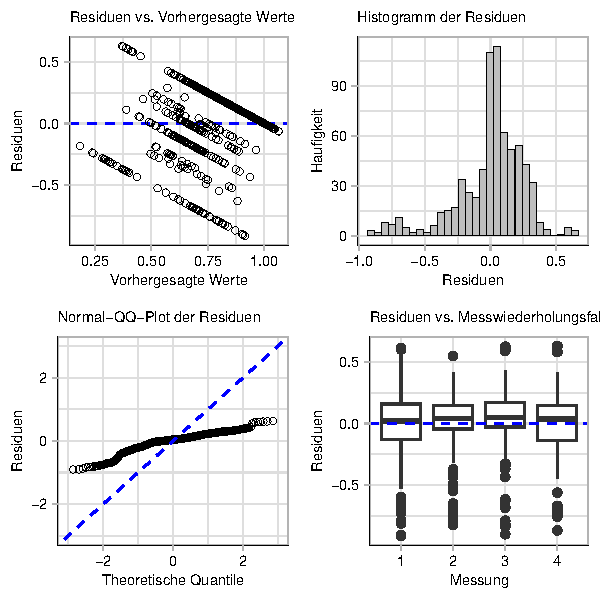
\includegraphics{lmm_vt-002}
%\input{plots/appendixtest.tex}

\end{center}
\caption{Residuen LMM Verkehrsteilnehmer}
\label{fig:one}
\end{figure}


\end{document}






